\chapter{Introduction to USB Power Delivery}

\section[Introduction]{\textbf{Introduction}}
The \gls{usb} has become the ubiquitous connector for data transfer and low-power device charging. However, traditional USB standards limited power delivery to 2.5W (USB 1.1) and 4.5W (USB 3.0) \cite{renesas_usb_pd}. This restricted the use of USB for charging power-hungry devices, such as laptops and tablets. To address this limitation, \gls{usbif} introduced the \gls{usbpd} specification \cite{usb_if_usb_charger}.

\gls{usbpd} is a game-changer, enabling significantly higher power delivery (up to 240W) through a single USB cable \cite{usb_if_usb_charger}. This is achieved by introducing intelligent negotiation between the power source and the device being charged. This negotiation allows for flexible voltage and current profiles, optimizing power delivery for various devices. Additionally, USB PD coexists with existing USB data communication standards, offering a unified solution for both data and power \cite{renesas_usb_pd}.

\gls{usbpd} emerged in 2012 alongside the USB-C connector (Fig. \ref{fig:typec_recep}). Prior to its introduction, charging speeds were limited by the USB Battery Charging specification. PD revolutionized this landscape by allowing devices to transfer higher power levels over a USB connection. With a single USB-C cable, it can deliver up to 100 watts of power, making it suitable for smartphones, tablets, and even laptops. The dynamic power negotiation ensures efficient and safe charging, while bi-directional capabilities enable scenarios like laptop-to-phone charging. 
\begin{figure}[htb]
\centering
	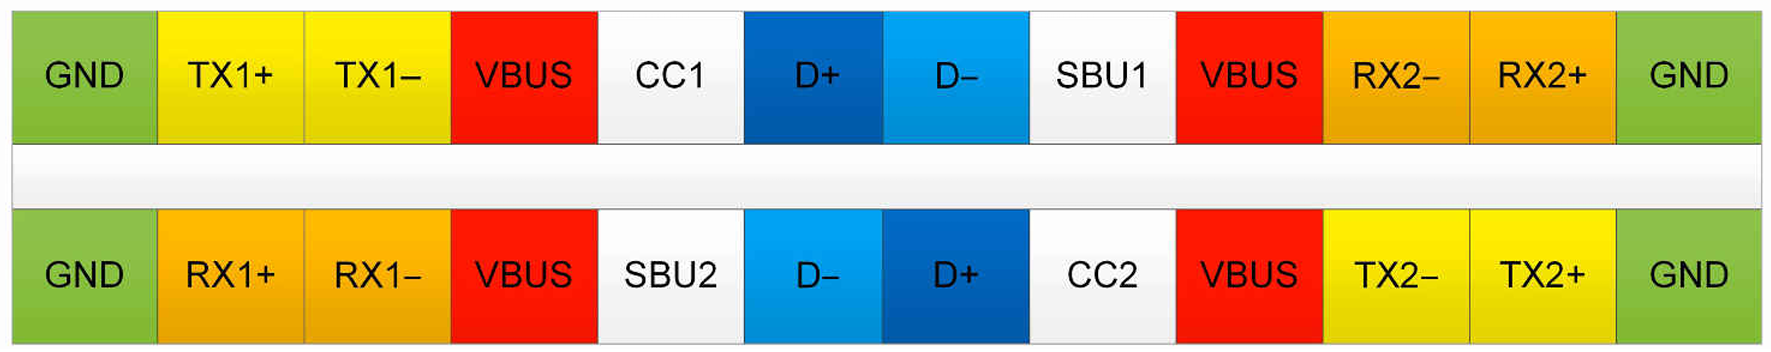
\includegraphics[scale=0.4]{Chapter1/Figures/typec_recep.png}	
	\caption{USB Type-C Receptacle }
	\label{fig:typec_recep}
\end{figure}

The heart of USB PD lies in the USB-C connector, a reversible interface that supports higher power levels. Devices communicate using power profiles to determine optimal power levels during charging. PD dynamically adjusts voltage and current, optimizing speed and safety. This technology has evolved over time, with USB PD 3.1 (released in 2021) supporting up to 240 watts, catering to a wide range of devices and high-power applications.

\section[Motivation]{\textbf{Motivation}}
USB PD enables devices to dynamically communicate their power needs. This ensures efficient and rapid charging by adjusting the power supply according to the device's requirements. USB Type-C connector is becoming ubiquitous due to its advantages: cost-effectiveness, backward compatibility with USB 2 and USB 3 standards, increased bandwidth, alternative modes (e.g., HDMI, DisplayPort), and durability.
%\vspace{0.5cm}
Implementing USB PD allows one to replace specialized connectors (e.g. barrel jacks) or built-in AC power sources. This reduction in components reduces the amount of electronic waste and reduces costs. Integrating both the PD controller and the power supply into a single chip using a \gls{bcd} node has the following advantages :-
\begin{enumerate}
    \item \textbf{Space Efficiency}: By integrating both components into a single chip, you can significantly reduce the overall footprint of your design. This is particularly beneficial for portable devices where space is at a premium.
    \item \textbf{Cost Reduction}: Integrated designs often lead to cost savings in the manufacturing process as they require fewer materials and less assembly.
    \item \textbf{Improved Performance}: With both components on the same chip, communication between the PD controller and the power supply can be faster and more efficient, potentially improving the overall performance of the system.
    \item \textbf{Power Efficiency}: An integrated design can also lead to improved power efficiency, as it reduces the power loss that can occur when signals travel between separate chips.
    \item \textbf{Reliability}: Having both components on a single chip can increase the reliability of the system by reducing the number of interconnections, which are potential points of failure.
\end{enumerate}
Ultimately, the motivation behind this project is to provide a potential solution to the demand for \gls{usbpd} applications that combines the advantages of advanced LDMOS technology with optimized circuitry and layout.
%\vspace{1cm}
\section[Problem statement]{\textbf{Problem statement}}

Efficiency, reliability, and compliance are major challenges in USB power delivery systems. Integrating a PD controller and power supply with these low parameters is essential.


\section[Objectives]{\textbf{Objectives}}
The objectives of the project are
\begin{enumerate}
\item To design and implement an \gls{usbpd} 3.1 compliant controller using CMOS Technology.
\item To design and implement an \gls{usbpd} 3.1 compliant Power Supply using BCD Technology.
\item To integrate the designed controller and Power Supply.
\item To evaluate performance metrics of the designed power supply such as transient response and stability and compare the proposed controller with existing designs in terms of performance and area.
\end{enumerate}

\section[Literature Review]{\textbf{Literature Review}}
\subsection{Overview of USB Power Delivery (USB PD)}
\subsection{The Role of Switching Regulators}
\subsection{Buck Converters}
\subsection{Flexible Voltage and Current Levels}
\subsection{Compliance with USB PD Standards}

\section[Brief Methodology of the project]{\textbf{Brief Methodology of the project}}
\begin{enumerate}
    \item \textbf{Designing the Circuit}: The first step is to design the RTL for PD controller and schematic entry for the power supply and its supporting circuitry.
    \item \textbf{Pre-layout AMS Simulation}: After the schematic design and RTL is complete, the next step is to perform a pre-layout AMS simulation of both devices using Spectre AMS. This involves applying the appropriate input signals to the circuit and observing the output signals. The simulation should verify that the circuit meets the desired performance metrics, such as output voltage, dropout voltage, current regulation, transient response, and stability.
    \item \textbf{Layout Generation}: After the pre-layout simulation confirms that the schematic design meets the desired performance metrics, the next step is to generate the layout of the power supply circuit using Cadence Virtuoso and controller through digital PNR flow. The layout should be designed in such a way that it minimizes the area of the circuit while maintaining the performance of the circuit. The layout should also take into account the design rules of the 45nm CMOS technology node.
    \item \textbf{Parasitic Extraction}: Once the layout is complete, the next step is to extract the parasitics of the circuit using Quantus RC. This involves identifying the parasitic resistances, capacitances, and inductances in the circuit that can affect the performance of the circuit. The extracted parasitics are then back-annotated to the schematic.
    \item \textbf{Post-layout AMS Simulation}: After the parasitics are back-annotated to the schematic, the next step is to perform a post-layout AMS simulation of the circuit using Spectre AMS. This involves applying the appropriate input signals to the circuit and observing the output signals. The simulation should verify that the circuit meets the desired performance metrics, taking into account the effects of the extracted parasitics.
    \item \textbf{Performance Evaluation and Comparison}: The final step is to evaluate the performance of the circuit and compare it with existing designs. This involves analyzing the simulation results and determining whether the circuit meets the desired performance metrics. The performance of the circuit should also be compared with existing designs in terms of performance and area to understand the impact of the CMOS technology node on the performance and area.
\end{enumerate}

This methodology provides a more comprehensive approach to designing and implementing an Integrated PD controller, taking into account both the schematic design and the physical layout of the circuit. It is designed to be comprehensible to both academia and industry professionals, and it provides a clear path from the initial design of the circuit to the final evaluation of its performance. 

\section[Assumptions made / Constraints of the project]{\textbf{Assumptions made / Constraints of the project}}

When designing a system with high power levels, it is crucial to protect the user and system from any harmful events that can happen on the power path. The most difficult event to protect against is a VBUS short to ground. In this instance, the current on VBUS will spike rapidly; it is up to the power path to open the FET immediately before it is damaged by these high current levels. If the FET does not open quickly enough, the spiked current can damage the FET and the rest of the system.

Many USB PD controllers on the market do not integrate the power paths. It is up to the hardware designer to implement protections using discrete components. 
 Implementing an overcurrent protection scheme discretely can be tedious; it usually involves using a sense resistor with a current-sense amplifier. The output of the current-sense amplifier is then fed into a comparator that will trigger a fault GPIO on the USB PD controller, or activate circuitry to disable the gate of the VBUS FET. 
 
This is not the best solution, as it’s not possible to adjust the overcurrent trip point once the comparator is set. In the event of a VBUS short to ground, it will take longer for a discrete solution to detect the short and open the FET than it would for the integrated power path to detect it.

In this work, \gls{pcl} is implemented. During overcurrent, the output voltage drops. Similarly, if VBUS shorts, the Gate-Source voltage of the PMOS pass element falls below \(Vthp\), turning off the PMOS.

\section[Organization of the report]{\textbf{Organization of the report}}

This report is organized as follows.  
\begin{itemize}
\item Chapter 2 discusses the fundamentals of \gls{usbpd}. 
\item Chapter 3 discusses the design of \gls{usbpd} controller and power supply.
\item Chapter 4 discusses the implementation of the design and the performance parameters for evaluation.
\item Chapter 5 discusses the results of tests used to validate the implemented design.
\item Chapter 6 discusses the conclusion and future scope of this project.
\end{itemize}

.